\section{Adversarial Distribution}

Our idea for the adversarial distribution is to test the ``early space management".

At each request we generate a residence with probability 80\% and a factory with probability 20\%.

For the residence, with half probability it's going to be a star-shaped, otherwise it's just a straight line.
The reason that we chose these two shaped is, we expected them to create a lot of empty ``holes" on the map, as
they couldn't fit each other nicely.

The factory part consists of two phases. During the first phase we generate 1x1 factories or 1x2 factories.
Then at certain point (after 140 rounds in our submitted version), it switches to second phase which produce
5x5 factories only.

We expect that the player should use small factories to fill the empty ``holes" that residences created instead of
place them into some ``empty areas". Otherwise during the second phase the player can hardly find enough empty areas
for giant 5x5 factories.

\begin{figure}[ht]
\centering
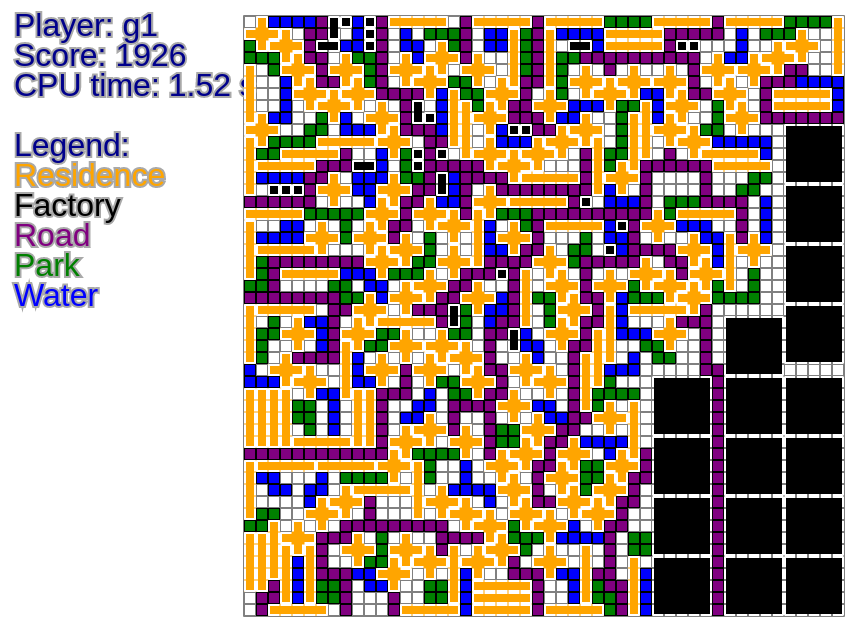
\includegraphics[width=0.8\textwidth]{IdealSolutionForAdversarial.png}
\caption{An `ideal' solution for this adversarial: let small factories
sneak into the residences area, which gives more freedom to the placement
of large factories}
\end{figure}
